\documentclass{standalone}
\usepackage{tikz}
\usepackage{ctex,siunitx}
\usepackage{tkz-euclide}
\usepackage{amsmath}
\usetikzlibrary{patterns, calc}
\usetikzlibrary {decorations.pathmorphing, decorations.pathreplacing, decorations.shapes,}
\begin{document}
\small
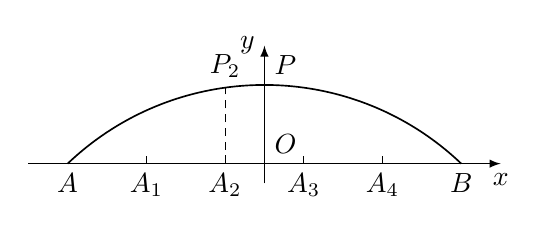
\begin{tikzpicture}[>=latex,scale=0.25]
  \draw[thin,->](-12,0)--(12,0)node[below]{$x$};
  \draw[thin,->](0,-1)--(0,6)node[left]{$y$};
  \tkzDefPoints{0/0/O,-10/0/A,10/0/B,0/4/P,0/-10.5/C}
  \tkzDrawArc[semithick](C,B)(A)
  \foreach \x[count=\i] in {-6,-2,2,6}
  {
    \draw[thin](\x,0)--++(0,0.4)node[at start,below]{$A_\i$};
  }
  \draw[densely dashed](-2,0)--++(0,3.86)node[above]{$P_2$};
  \tkzLabelPoints[above right](O,P)
  \tkzLabelPoints[below](A,B)
\end{tikzpicture}
\end{document}